\section{Arduino Support}
Going into the software design scheme, some considerable useful library support would be those from the Arduino platform. 
Before software implementation, the main hardwares parts were chosen for this project. More detail on the parts choices
will be explained in the next chapter. 
Since the micro controller unit (MCU) and transceiver module are decided to be Arduino Nano with chip model ATMEGA328 and 
chip model CC1101, the three libraries of the testbed built out of are \texttt{<Arduino.h>}, \texttt{<EEPROM.h>} and \texttt{<ELECHOUSE\_CC1101.h>}. 
In the Arduino header file, there are lists of Digital, Analog and Advanced input/output (I/O) functions that are pre-built
for programmer uses \cite{arduino_reference}. It also declares standard scopes of the data types and the constants.
The Arduino library gives full access of the fundamental control structure, such as ``loop'', ``if'', ``return'' statements,
etc. Above categories are some of the handy functions that have been used in the CR testbed. Next, to keep track of the 
emulation result, each CR device will need to record some important occurrences during the experiment somewhere.
The built-in electrically erasable programmable read-only memory (EEPROM) in Arduino Nano is a great place to store data. \texttt{<EEPROM.h>} includes all the basic
functions that the project needs within the library. Lastly, the project utilizes
the \texttt{<ELECHOUSE\_CC1101>} files by developer, Michael, from Elechouse Company. It provides basic subroutines
for parameterizing the CC1101 transceiver chip as it communicates with the MCU. 
In Github, username, Little Satan, modified a much more user friendly version of the Library called, 
\texttt{SmartRC-CC1101-Driver-Lib}. It further develops sets of classes and functions, leaving users an easy setup
at a high level abstraction; that is, the transceiver library this project is using. Below are few lines of code in 
the programming scripts when referencing the tools.
\newline
\begin{lstlisting}[caption={Library used in the testbed},captionpos=b]
// Include Libraries
#include <Arduino.h>
#include <EEPROM.h>
#include <ELECHOUSE_CC1101_SRC_DRV.h>
\end{lstlisting}


The overall structure of the testbed is built using the Arduino library. To get access to all common constants value easier, 
it initializes the numbers in the header files. Arduino platform allows the building and use of custom library, which users can take advantage
of, making a much more suitable subroutine for specific operation. One other function that the testbed uses for device performance indication 
is the LED manipulation in the digital general purpose input output (GPIO) port. The way it records data is by storing to the build-in
EEPROM inside the ATMEGA328 chip. It monitors data through 
serial peripheral interface (SPI) communication between the CR device and the graphical user interface (GUI) within the client machine.
In \texttt{<ELECHOUSE\_CC1101\_SRC\_DRV.h>} and related compiled files, modified functions provide direct manipulation from MCU 
to CC1101 chip through SPI as well. The handy functions convert user level instructions to digital signals, which then also be transferred 
through SPI. With every data retrieval MCU can react based on sensed value. The summary of the functions used are included in
Table~\ref{tab:function}, Table~\ref{tab:function2} and Table~\ref{tab:function3}.

\section{Protocol Setup}

This testbed emulates operational and authentication methods that radios use in the air. During the experimental process, 
the Base Station (BS), Customer Premises Equipments (CPE) and Licensed Band Users (LBU) communicate and interfere using 
a set of specific protocols. They send messages through custom packets one after another to simulate frames. The testbed simplified 
the process by encoding four fields in a packet, the operational code, payload, source ID and destination ID, as Figure~\ref{fig:packet} describes. 
Each field is 8 bits or 1 byte long. The message packet in total is 4 bytes in length. The operational code is responsible for identifying the 
action that the device is taking, as well as the device type. In the payload section, it functions differently with a different operational code.
The source ID and the designation ID usually refers to the message packet itself. For the full set of message structures and their functions, 
please refer to Table~\ref{tab:structure}.


\begin{figure}[ht]
\centering
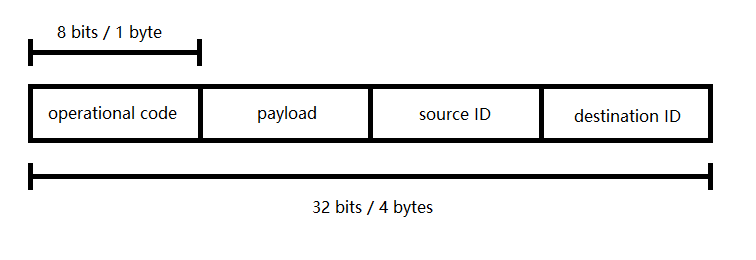
\includegraphics[width=12cm]{figures/packet.png}
\caption{Message Packet Structure}
\label{fig:packet}
\end{figure}

Some of the communication scenarios will be discussed below. When a CPE wants to setup a connection with another CPE, the device needs to 
identify its actions by putting a corresponding operational code, a number indicating desired connection duration, its own user ID number, and 
the target user ID number. It sends at the reserved channel and waits for a response back from BS, the centralized unit of the network, until the timer expires. 
\begin{figure}[ht]
  \subfloat[Perfect Connection Setup]{
	\begin{minipage}[c][1.5\width]{
	   0.4\textwidth}
	   \vspace{-14mm}
	   \centering
	   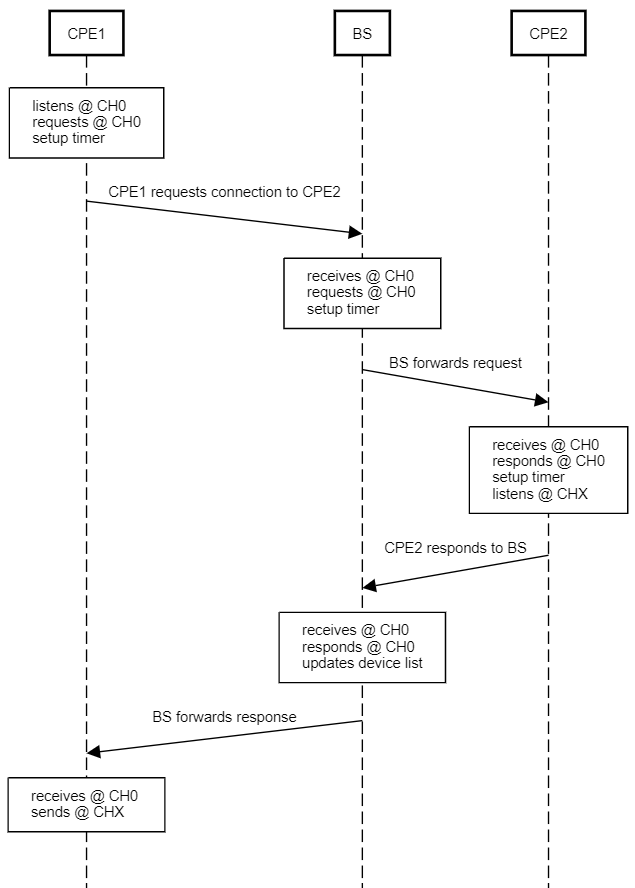
\includegraphics[width=0.8\textwidth]{figures/sequence_diagram_perfect_com.png}
	\end{minipage}}
 \hfill 	
  \subfloat[Message Dropped at the 1st Transmission]{
	\begin{minipage}[c][1.5\width]{
	   0.4\textwidth}
	   \centering
	   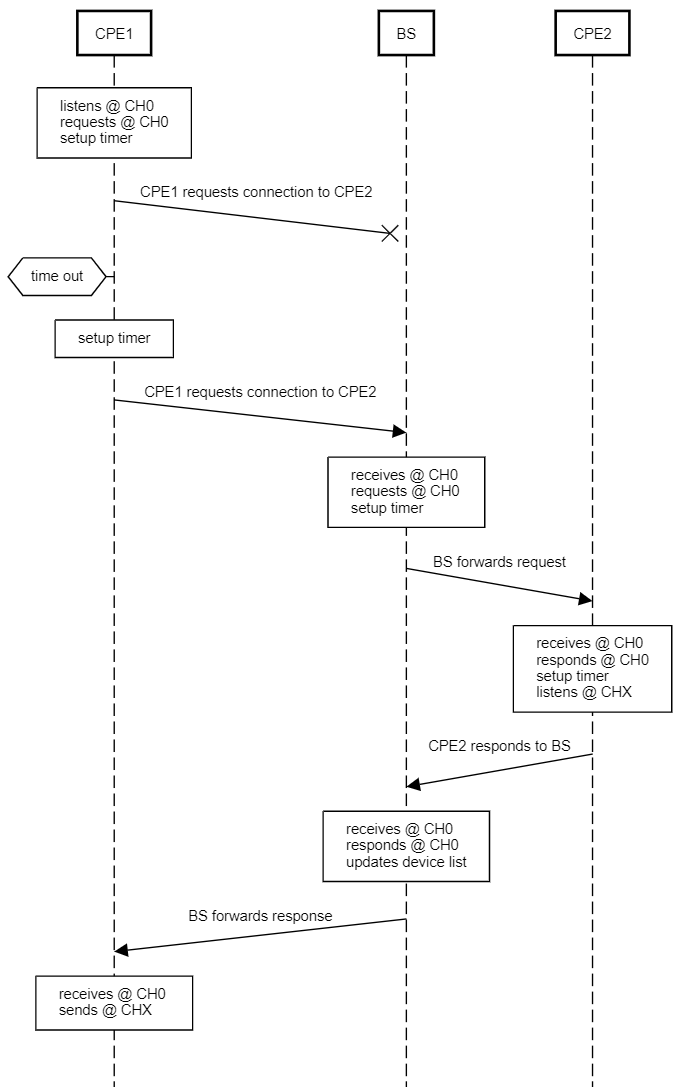
\includegraphics[width=0.85\textwidth]{figures/sequence_diagram_first_miss_com.png}
	\end{minipage}}
\caption{Connection Setup}
\label{fig:connection_setup}
\end{figure}


BS catches the messages and decodes them, which could be further processed by program logic. BS then forwards the message to the target
CPE by inserting an assigned channel to the payload field. After transmitting, BS sets up a timer and waits for a response. As the target
device receives a request from BS, it responds right back with a corresponding operational code and confirms the channels with the same payload
information as the incoming message. Note, that in this packet, the source ID will be the target CPE and the destination ID will be the 
original requesting CPE ID. BS catches the response; it forwards back to the requesting CPE to let it know that the connection has been set up
successfully. A perfect scenario is demonstrated by the sequence diagram in Figure~\ref{fig:connection_setup}(a). However, if the initial 
request could not reach to BS by the time the timer expires, the source CPE would send another request until it receives a desired response from
BS. Figure~\ref{fig:connection_setup}(b) shows a successful connection after the first transmission miss. If the connection process is interrupted or
any of the devices could not catch the response, like those sequence diagrams shown in Figure~\ref{fig:other_miss_cases}, the source CPE would have to try the whole process again when the timer expires.

\begin{figure}[ht]
  \subfloat[Message dropped at the 2nd]{
	\begin{minipage}[c][1.4\width]{
	   0.31\textwidth}
	   \vspace{-20.5mm}
	   \centering
	   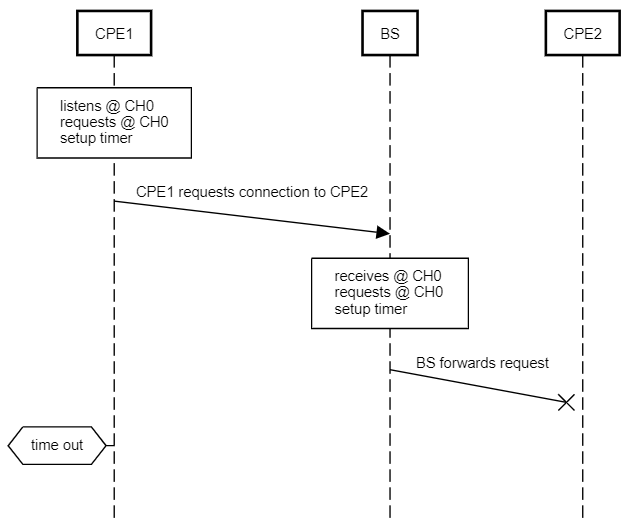
\includegraphics[width=1\textwidth]{figures/sequence_diagram_second_miss.png}
	\end{minipage}}
 \hfill 	
  \subfloat[Message dropped at the 3rd]{
	\begin{minipage}[c][1.4\width]{
	   0.31\textwidth}
	   \vspace{-13mm}
	   \centering
	   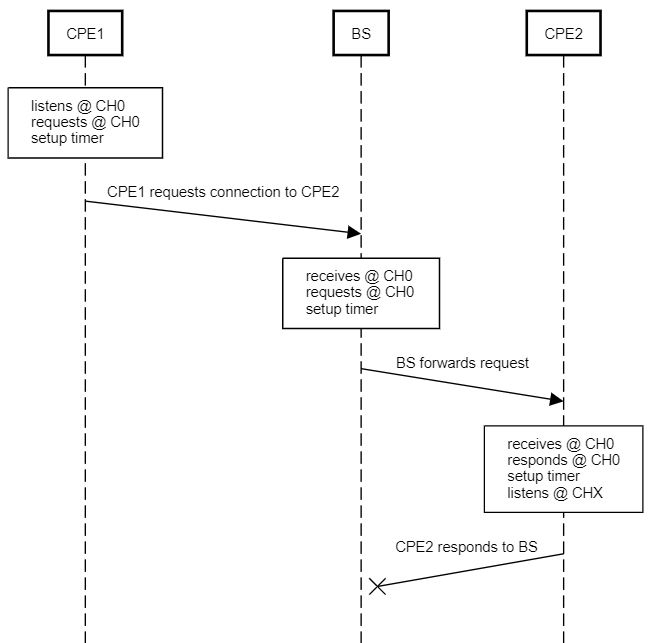
\includegraphics[width=1\textwidth]{figures/sequence_diagram_third_miss.png}
	\end{minipage}}
 \hfill	
  \subfloat[Message dropped at the 4th]{
	\begin{minipage}[c][1.4\width]{
	   0.31\textwidth}
	   \vspace{0mm}
	   \centering
	   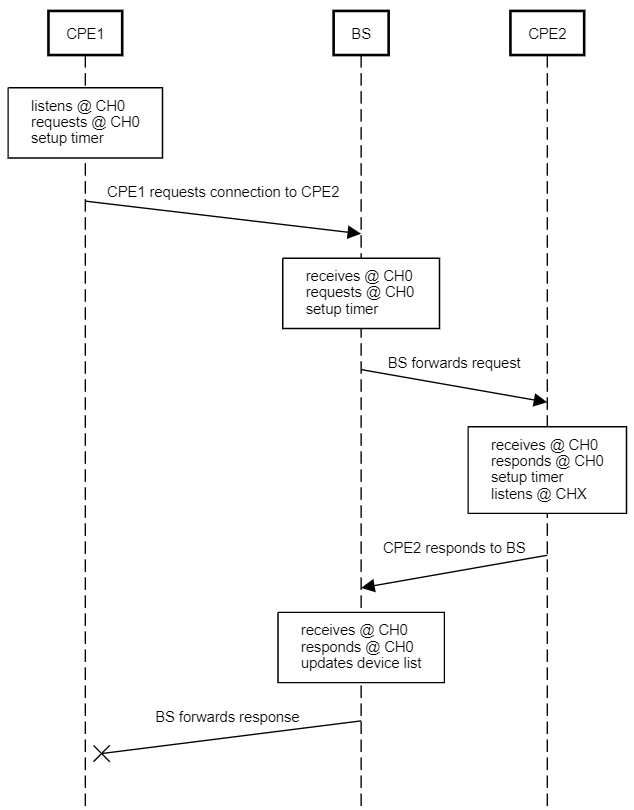
\includegraphics[width=1\textwidth]{figures/sequence_diagram_fourth_miss.png}
	\end{minipage}}
\caption{Other Miss Cases}
\label{fig:other_miss_cases}
\end{figure}

Upon establishing a connection, two CPEs would send and receive data at a designated channel that is different from the reserved channel. A successful data transfer results in both CPEs returning to the reserved channel normally shown in Figure~\ref{fig:with_lbu}(a). During the data transfer period, if any LBU happens to transmit at the frequency that CPEs are at, both CPEs are forced to drop the in progress communication at the current channel, like the one in Figure~\ref{fig:with_lbu}(b). A new channel connection is required to be set up. 



\begin{figure}[ht]
  \subfloat[Successful Data Transfer]{
	\begin{minipage}[c][1.7\width]{
	   0.4\textwidth}
	   \centering
	   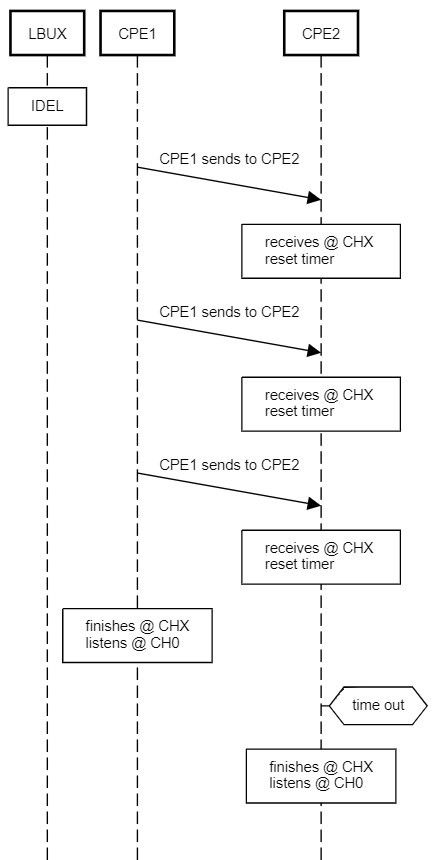
\includegraphics[width=0.8\textwidth]{figures/sequence_diagram_no_interrupt.png}
	\end{minipage}}
 \hfill 	
  \subfloat[Data Transfer Interruption]{
	\begin{minipage}[c][1.7\width]{
	   0.4\textwidth}
	   \vspace{-33mm}
	   \centering
	   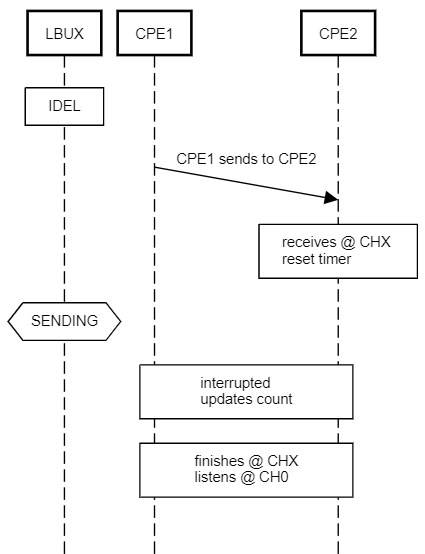
\includegraphics[width=0.8\textwidth]{figures/sequence_diagram_interrupt.png}
	\end{minipage}}
\caption{With Licensed Band Users}
\label{fig:with_lbu}
\end{figure}

\section{Establish Library}

The benefits of establishing specific libraries are making both the repetitive, complex logic easier to use and the process more scalable. 
Each library comprises of two files, a header file with all the defined functions and a C++ file that codes in all the logics. Some constants are 
also defined in the header file. These libraries generally help project development in the long run. 
Next, are the two customized libraries, \texttt{RADIO} and \texttt{TEST}, that were made and included in this testbed. For the full description of operational code constants in the header files, please refer to Table~\ref{tab:structure}.

\subsection{RADIO}
\texttt{RADIO} library integrates those necessary subroutines to manipulate the transceiver module into short accessible function calls. Notice that the project avoids channel interference by defining a large channel separation. \texttt{switchChannel(byte)} subroutine makes sure it switches to the correct frequency. To understand and use all functions in this library, follow the method descriptions and formats that are listed below.

\begin{itemize}
  \item \texttt{void initialize\_trans(void)}\newline
  Description: it sets up initial parameters for the CC1101 registers, using some of the \texttt{ELECHOUSE\_CC1101\_SRC\_DRV} functions, including transmission mode, transmission modulation, base frequency, receiver bandwidth, etc.\newline
  Format: input NONE; output NONE.
  \item \texttt{void receiveMessage(int, byte *, byte, byte)}\newline
  Description: it utilizes \texttt{CheckRxFifo()} and \texttt{CheckCRC()} from \texttt{ELECHOUSE\_CC1101}. Based on user defined device type and target ID, when the corresponding flag is raised, it retrieves the data in the air and decodes the message, and then puts it back to the message placeholder at the end.\newline
  Format: input receive maximum duration, received message placeholder, device type and target ID; output NONE.
  \item \texttt{void sendMessage(int, byte *)}\newline
  Description: it encodes the message in the input placeholder and sends it to the air throughout the duration time period.\newline
  Format: input transmit duration and transmit message placeholder; output NONE.
  \item \texttt{void switchChannel(byte)}\newline
  Description: it switches channels by modifying CC1101 registers based on the defined channel separation.\newline
  Format: input channel number; output NONE.
  \item \texttt{void encode(byte *, byte *)}\newline
  Description: it merges packet fields into a condensed buffer for transmission in the air.\newline
  Format: input packet message separated in fields; output condensed packet data.
  \item \texttt{void decode(byte *, byte *)}\newline
  Description: it decodes the condensed data stream into logical processable packet fields. \newline
  Format: input packet raw data buffer; output packet message separated in fields.
\end{itemize}




\subsection{TEST}
\texttt{TEST} library is made for generalizing most of the CR testing environment setup. In the header file, the user should put all of the test cases and stimulus. The constants defined at the top of the file apply to the current experiment, such as the schedule size, emulation duration, algorithm type, number of devices under test (DUT), etc. There are also handy subroutines developed for recording and monitoring the data. To understand and use all functions in this library, follow the method descriptions and formats that are listed below.

\begin{itemize}
  \item \texttt{void initialize\_scheduleList(byte, byte *)}\newline
  Description: it places the schedule in the LBU programs for them to follow accordingly.\newline
  Format: input LBU ID and schedule array placeholder; output NONE.
  \item \texttt{void record(int, byte, byte)}\newline
  Description: it first stores time and then data to the given memory location.
  Format: input memory location, time data and value data; output NONE.
  \item \texttt{void report(void)}\newline
  Description: it displays all data from the memory to the monitor in the client machine.\newline
  Format: input NONE; output NONE.
\end{itemize}

\section{Program Module}

This section goes into the software flow of each individual type of device. During physical testing, BS, CEPs and LBUs first establish a regional network shown in Figure~\ref{fig:network}. For this testbed, all devices communicate through broadcasting, especially the BS. CPEs are software defined as enabling point to point, which means two CPEs can talk to each other without the BS in the middle after the channel is established. The LBUs interrupt also in a broadcasting way. The primary and the secondary devices interact with each other based on the testing stimulus or the assigned tasks. Some outcomes of the interaction would be recorded individually by the CPEs. To explain their operating relationship and the flow of the program, it includes state-diagram-level abstractions on how they run in the experiment. The complete code of the project is included in this link: \newline \url{https://github.com/SaltFishBoi/cognitive_radio_network_environment_deployment} 

\begin{figure}[ht]
\centering
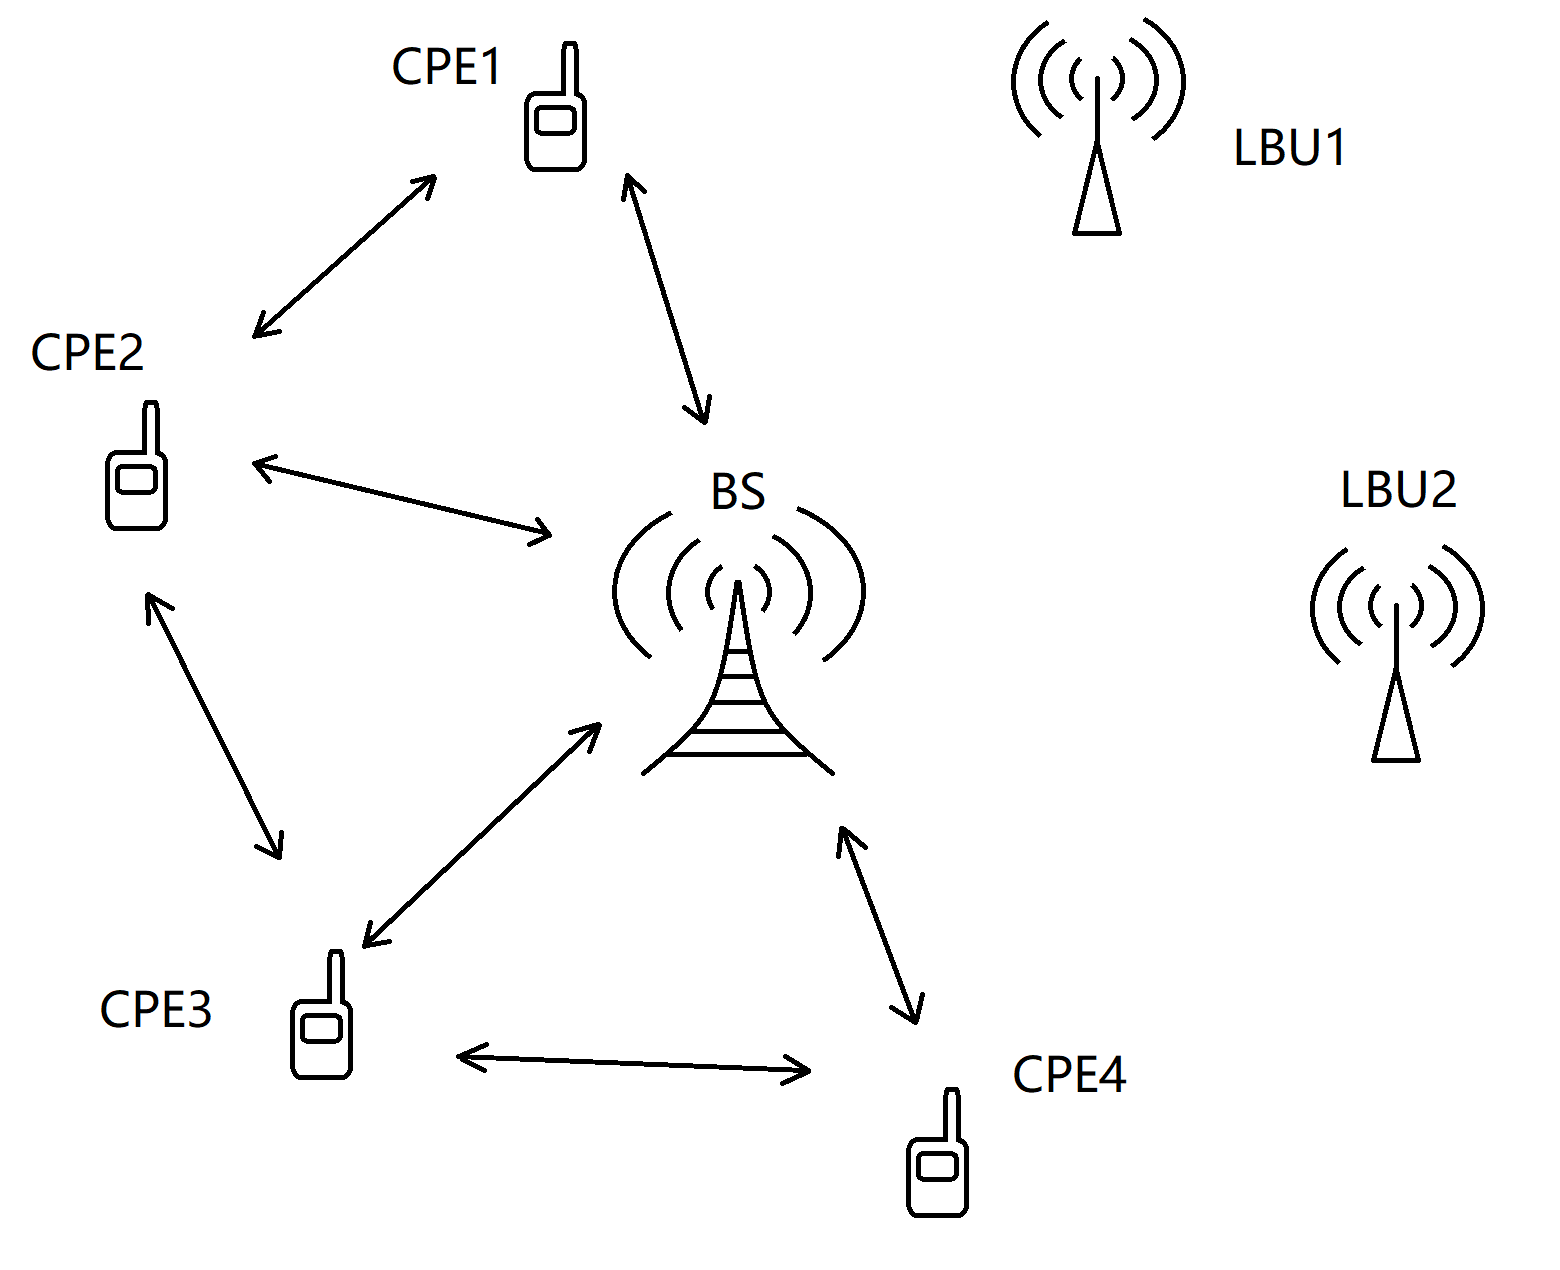
\includegraphics[width=12cm]{figures/network.png}
\caption{Cognitive Radio Regional Network}
\label{fig:network}
\end{figure}


\subsection{Base Station}

The centralized unit for CRN is BS. It is responsible for sensing the environment and overseeing the spectrum assignment. The station starts by setting all necessary indicators and register values for the transceiver module. Next it initializes all the tables, a mechanism that keeps track of the changing environment. The tables include the spectrum table, client table, and the selection table for more advanced algorithms. The experiment requires every device under the test to be synchronized in time. Being the central unit of the network, the BS needs to synchronize the time with the rest of the devices in the next step. After that, the program performs the main process, which can be described by the state diagram shown in Figure~\ref{fig:state_diagram_bs}. The BS is running in two states, listening to any incoming request and responding to a request. During the listening state, it relies on the functions in \texttt{RADIO} library to retrieve messages sent from CPEs in the air. Once it receives a valid request from a CPE, it goes to responding state, based on the algorithm specified in the test. It selects the corresponding channel and sends that request to the target CPE. It then waits for a response back from the same CPE with the target ID. If it never catches the response from the target CPE, it will go back to the listening state as if the message had been dropped. If it catches a response from the target CPE, it would update the client list status because two CPEs would be talking soon. Upon sending a response back to the source CPE, the BS has created a successful connection and will go back to the listening state. Based on the algorithm requirement, the BS senses the environment and updates the selection table periodically.

\begin{figure}[ht]
\centering
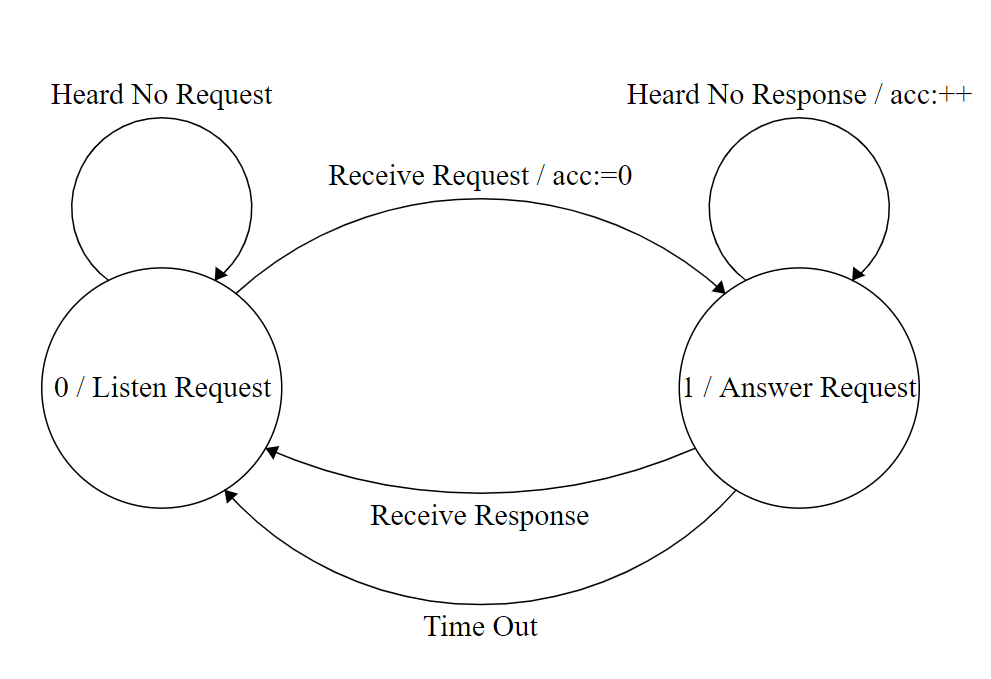
\includegraphics[width=12cm]{figures/state_diagram_bs.png}
\caption{State Diagram Base Station}
\label{fig:state_diagram_bs}
\end{figure}


\subsection{Customer Premises Equipment}
All secondary devices, CPEs, need to first set the indications and register values for the transceiver modules as well. Next in the CPE program, it synchronizes with the BS. After that, in the CPE main process loop, it runs at one of three states as shown in Figure~\ref{fig:state_diagram_cpe}. All CPEs initially try requesting BS for a connection to another CPE. If the BS picks up the message and responds back with an assigned channel before the request timer expires, the source CPE would hop into the assigned channel and begin sending data. Then CPE sender would be done sending if it goes through the whole scheduled duration without interruption. The sender is capable of sensing if the channel is busy, in which LBU occupies the channel. It returns back to the request state if any of the two cases occurs. The occurrences would be accumulated and stored in the memory.

\begin{figure}[ht]
\centering
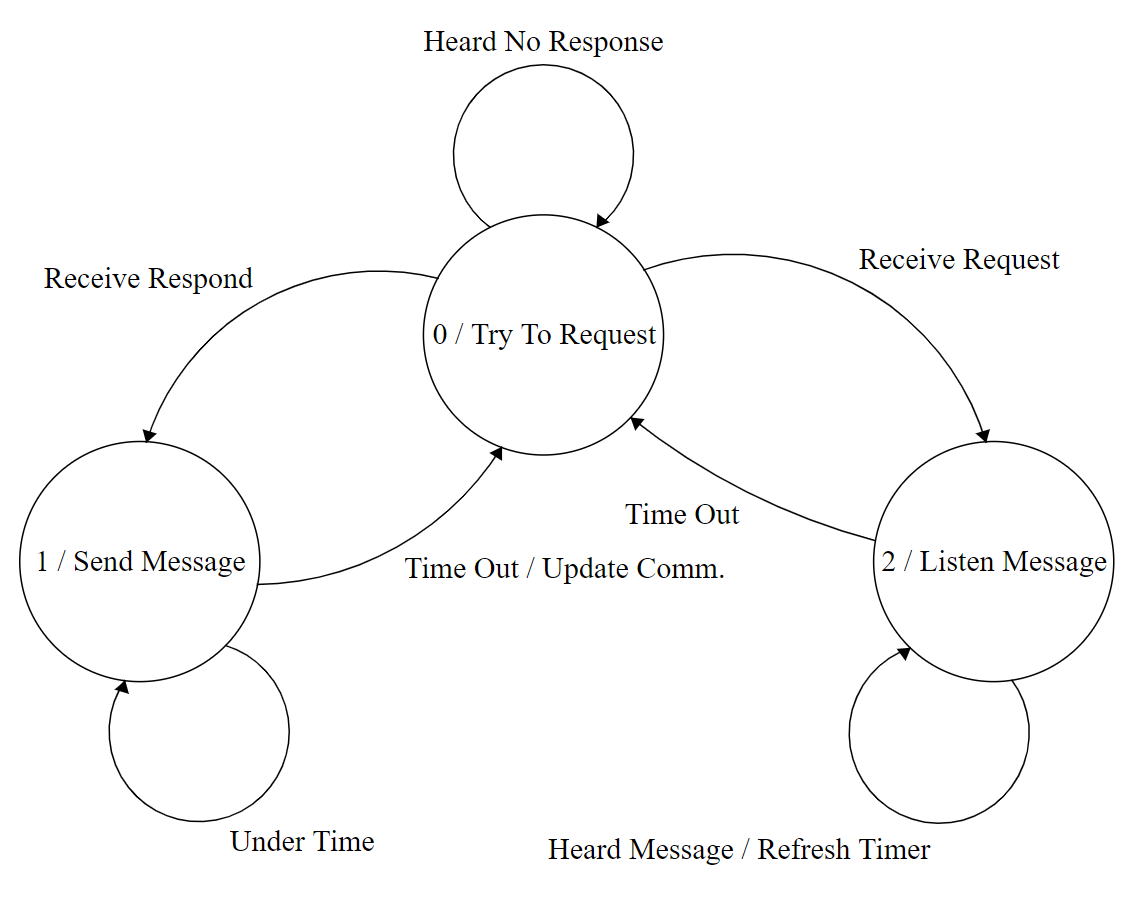
\includegraphics[width=14cm]{figures/state_diagram_cpe.png}
\caption{State Diagram Customer Premise Equipment}
\label{fig:state_diagram_cpe}
\end{figure}

If CPE hears nothing back from BS that is associated with its ID throughout the request time period, CPE will send the request again after a constant time of delay. During the requesting process, if CPE hears a connection request from another CPE forwarded by BS, it would confirm the channel and respond back to BS. In this case, it will hop into the assigned channel and go into the listening state. In that channel, it sets and refreshes a listening timer everytime it hears back from the CPE sender. It will go back to the request state when the timer expires or the channel is busy. 

The CPE finishes the process by taking the user defined experiment time into account. It emulates the real time, days and weeks in a much shorter period. By the end day that is set for the experiment, the CPE main process exits and the test is finished.  

\subsection{Licensed Band User}

LBU devices act as spectrum interrupters in this testbed. Again, LBUs need to first synchronize with all the rest of the device. After that, it initializes schedules with the \texttt{TEST} library. Based on the schedule and current synchronized time, LBU sends data at the designated channels. It loops the process until the experiment is done.


\begin{figure}[ht]
\centering
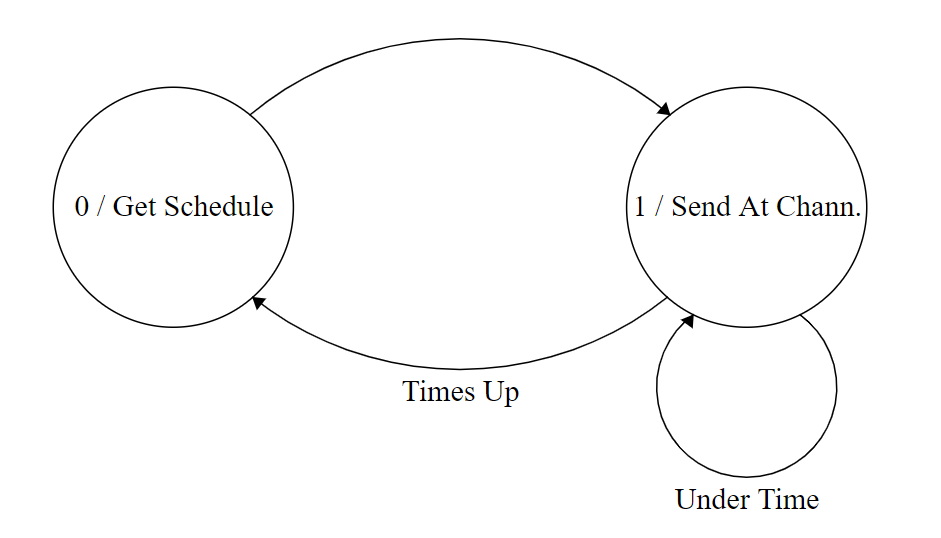
\includegraphics[width=12cm]{figures/state_diagram_lbu.png}
\caption{State Diagram Licensed Band User}
\label{fig:state_diagram_lbu}
\end{figure}